\documentclass{article}

\usepackage{amsmath}
\usepackage{graphicx}
\usepackage{listings}
\usepackage{color}


\usepackage{xepersian}
\settextfont{BNazanin} 
\linespread{1.3}
\newcommand{\linia}{\rule{\linewidth}{0.5pt}}

\def\LOGO{
\begin{picture}(0,0)\unitlength=1cm
\put (0.5,0) {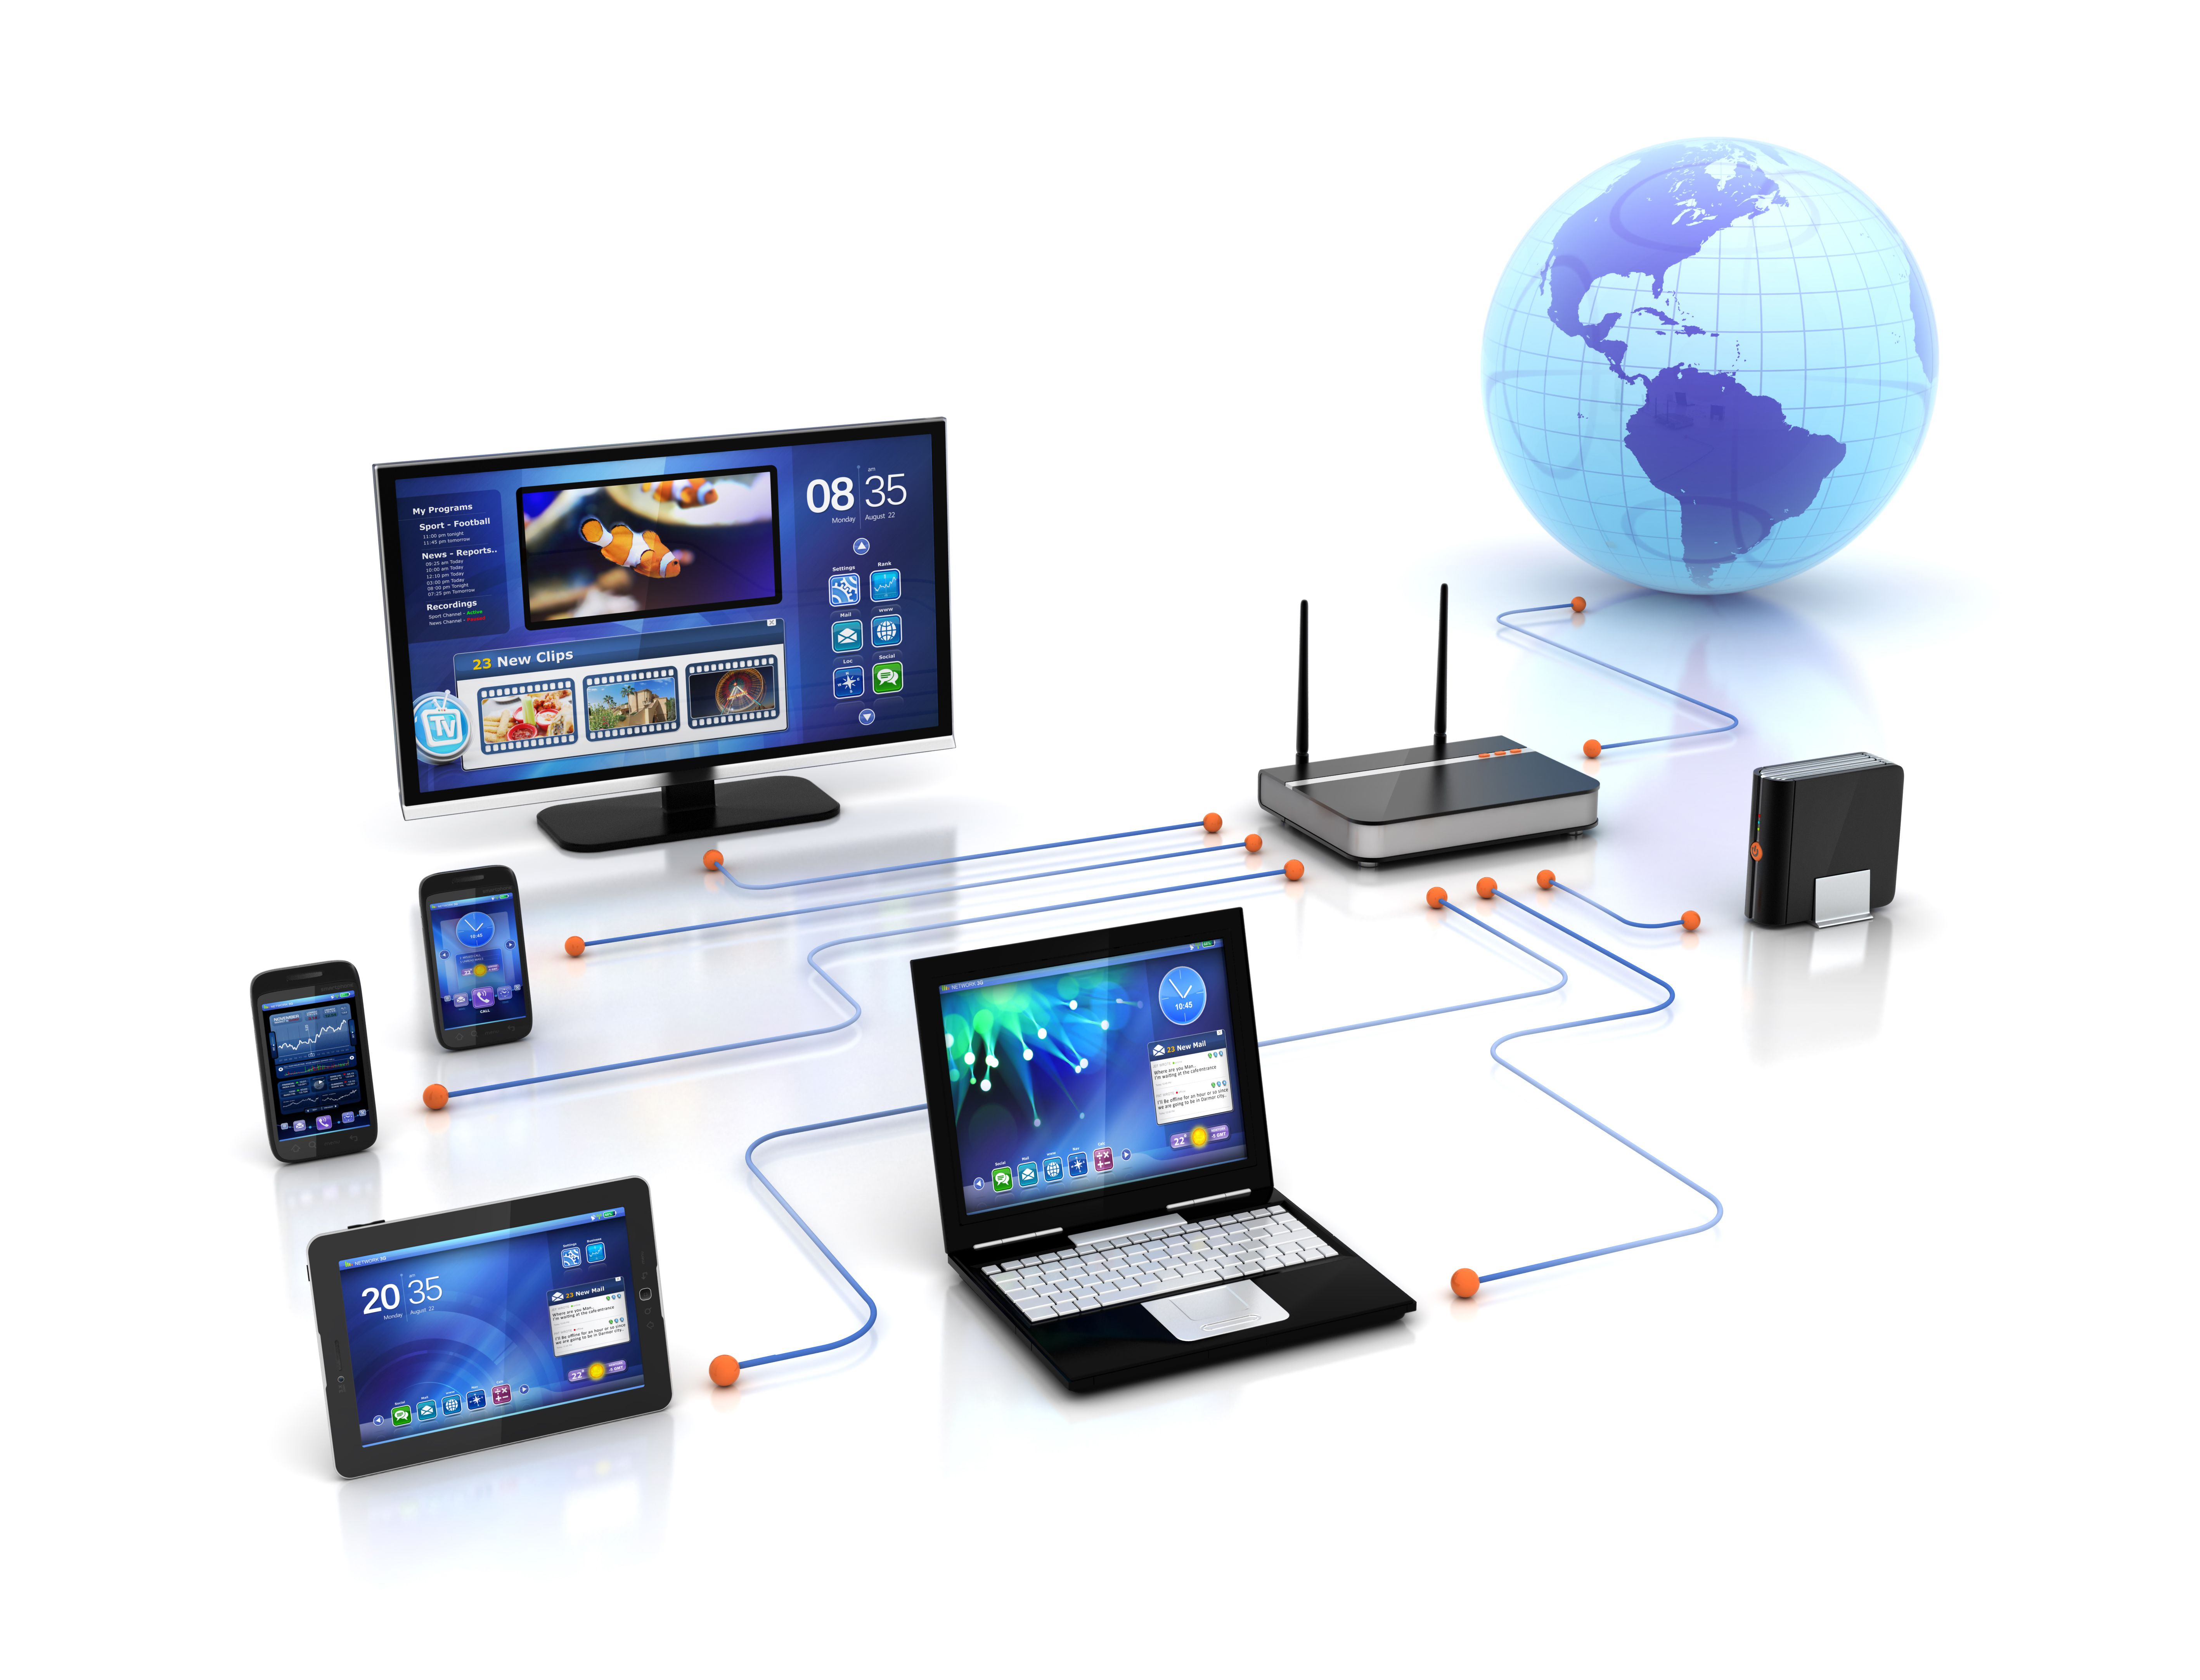
\includegraphics[width=5.1em]{network.jpg}}
\end{picture}
}

\def\LOG{
\begin{picture}(0,0)\unitlength=0.5cm
\put (-6,0) {
\includegraphics[width=4em]{question.png}}
\end{picture}
}

\definecolor{mygreen}{rgb}{0,0.6,0}
\definecolor{mygray}{rgb}{0.5,0.5,0.5}
\definecolor{mymauve}{rgb}{0.58,0,0.82}

\lstset{ 
  backgroundcolor=\color{white},   % choose the background color
  basicstyle=\footnotesize,        % size of fonts used for the code
  breaklines=true,                 % automatic line breaking only at whitespace
  captionpos=b,                    % sets the caption-position to bottom
  commentstyle=\color{mygreen},    % comment style
  keywordstyle=\color{blue},       % keyword style
  stringstyle=\color{mymauve},     % string literal style
}


\begin{document}

\title{\LOG        سوال ۱ کلاس استاد        \LOGO }
\author{نازنین صبری\\۸۱۰۱۹۴۳۴۶}
\date{ ۱۲ اسفند ۱۳۹۶}
\maketitle

\renewcommand{\labelenumii}{\alph{enumii}}
\begin{enumerate}
	\item  نرخ چیست؟\\نرخ به طور کلی ترجمه‌ی کلمه‌ی \lr{rate} است.\\ \lr{transmission rate}: زمانی که به بررسی اینترنت با دیدگاه پیچ و مهره می‌پردازیم بیان شده است که هاست‌ها با استفاده از لینک‌های ارتباطی \lr{(communicaton links)} و \lr{packet switch} ها به هم وصل شده اند که این لینک‌های ارتباطی می‌توانند داده‌ها را با سرعت‌های مختلف از خود عبور دهند که این سرعت انتقال \lr{transmission rate} دارد و با واحد بیت در ثانیه اندازه‌گیری می‌شوند. پس نرخ به معنی تعداد بیت‌های عبور کرده از لینک ارتباطی در هر ثانیه است. \\در صفحه ۱۹ اسلاید درباره‌ی نحوه‌ی‌ ارسال اطلاعات توسط هاست گفته شده است و توضیح داده شده است که پیام گرفته شده از برنامه به تکه‌های کوچکتری به نام پکت شکسته می‌شود که این پکت‌ها طول \lr{L} دارند یعنی از \lr{L} بیت تشکیل شده اند و به داخل شبکه ای با \lr{transmission rate R} فرستاده می‌شوند که در این صورت تاخیر \lr{transmission} برابر خواهد بود با \lr{L/R} ثانیه. در خلال این توضیح بیان شده است که نام‌های دیگر \lr{transmission rate} عبارتند از: \lr{link capacity} و یا \lr{bandwidth}\\\lr{bandwidth}: مقدار داده‌ای که می‌تواند در یک بازه زمانی مشخص منتقل شود. (از یک نقطه به نقطه دیگری برده شود) که این مدت زمان مشخص معمولا یک ثانیه است و مقدار داده نیز اغلب با واحد تعداد بیت بیان می‌شود. 
	\item در \lr{queuing delay} چرا \lr{La/R} نباید به یک برسد یا از آن بیشتر شود؟\\در حالت کلی می‌دانیم که \lr{R} مقدار \lr{transmission rate} است یعنی نرخ خارج شدن بیت‌ها از صف. \lr{a} نرخ متوسط رسیدن (وارد شدن) پکت‌ها به صف است واحد آن تعداد پکت در ثانیه است و \lr{L} تعداد بیت‌‌های پکت‌ها است. بر اساس متن کتاب نسبت \lr{La/R} با نام شدت ترافیک شناخته می‌شود. \\ علت اینکه این نسبت نباید به ۱ یا بیشتر از آن برسد این است که ۱ یا بزرگتر از ۱ بودن این نسبت به این معنی است که نرخ متوسط وارد شدن بیت‌ها در صف بیشتر از نرخ خروج (انتقال) بیت‌ها است، که این اتفاق باعث می‌شود که صف ایجاد شده همواره در حال افزایش باشد و به هیچ روش امکان کم شدن طول این صف در زمان وجود ندارد چون همواره به طور متوسط میزان ورودی بیشتر است و خروجی جواب‌گو نخواهد بود که این اتفاق باعث می‌شود که در طی زمان طول صف ایجاد شده در ورودی به سمت بی‌نهایت میل کند. برای جلوگیری از ایجاد این صف به طول بی‌نهایت (در دنیای واقعی چون امکان ایجاد حافظه کافی برای صفی به طول بی‌نهایت نیست در واقع برای جلوگیری از \lr{loss} که به بی‌نهایت میل می‌کند) به عنوان یک قانون در نظر گرفته می‌شود که نسبت \lr{La/R} نباید ۱ یا بزرگتر از ۱ بشود.\\
	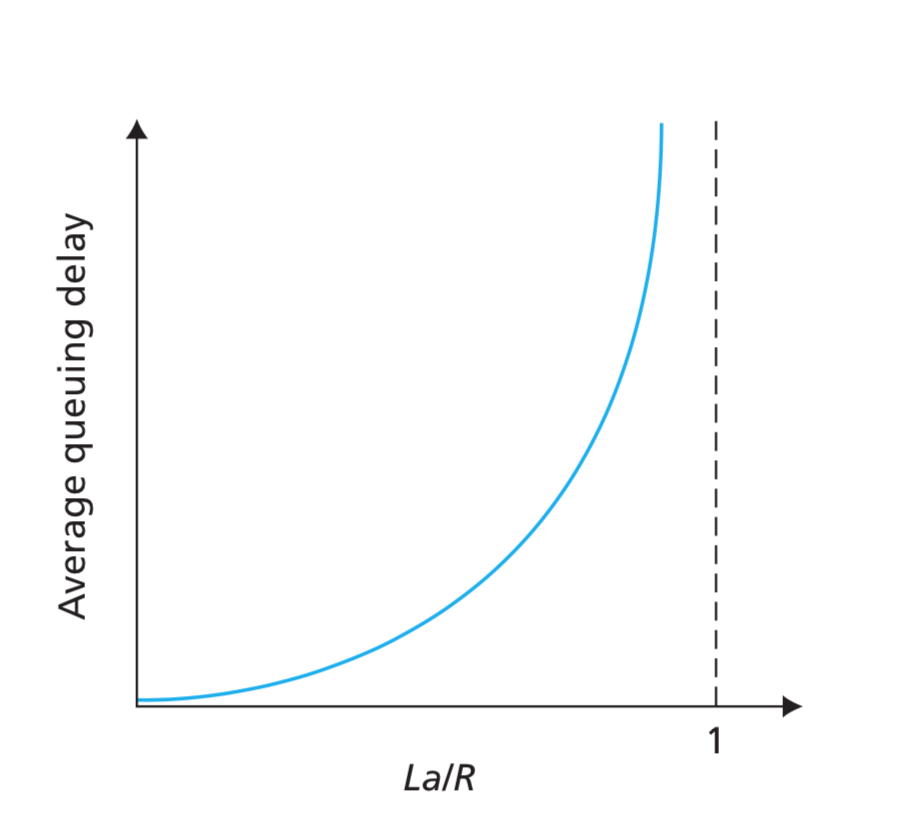
\includegraphics[scale=0.6]{./delay} 
\end{enumerate}


\end{document}